%%%%
%% Development :: User Interface
%%%
\section{User Interface}
\label{sec:imp_user_interface}

In order for users to use the system a simple and powerful user interface was 
required. The design reasonings behind the user interface were described in 
the design section.

The user interface has been designed utilising a fall-back system, which is a 
standard web development approach. The majority of the user interface is 
delivered by the server utilising JavaServer Pages (JSP) language.

The JSP language essentially extends from XML, and allows for html-like code to 
be written so that when compiled with Java, a full server-side page is rendered.
Within this project an additional JavaServer Pages Standard Tag Library was 
used. The library -- xml -- provided additional functionality so that JSP was 
able to directly utilise XML within its rendering technique.

Figure \ref{xmlOutput} illustrates an example XML parsing snippet from the 
\texttt{solver.jsp} file.

\begin{lstlisting}[language=XML, 
                   caption={isPatternValid deduces if a given solution pattern 
                            is valid}, 
                   label=xmlOutput] 
  <x:choose>
    <x:when select="$solution/trace">
      <p>Solution Trace:</p>
      <ol>
        <x:forEach select="$solution/trace" var="trace">
          <li><x:out select="$trace"/></li>
        </x:forEach>
      </ol>
    </x:when>
    <x:otherwise>
      <p>Solution Trace Unavailable.</p>
    </x:otherwise>
  </x:choose>
\end{lstlisting}

The code snippet above shows use of the XML library, as denoted by the 
`\texttt{x}' name space to certain elements. The code is utilising XPATH to find
all possible traces that are listed within the trace element (the trace element 
is an array).

For each of the traces found they will be printed out into the standard HTML 
output. However if a solution has not been found a simple predefined message 
will be presented.

The server side rendering that has been described above is known as the 
fall-back option. This option will work on all browsers and operating systems. 
The reason for this is that the rendering is controlled by the server, and hence
can be fully tested.

Many modern browsers will support JavaScript in some form of fashion. This 
allows for various additional functionality to be provided to enhance the user's
web browsing experience.

The cryptic crossword website features a JavaScript override that will override
the default server-side rendering and provide its own rendering. For example
when a user clicks upon the `solve' button, the website will display a message
informing the user that the clue is currently being solved as shown in figure 
\ref{fig:solving_clue_message}. Under a non-JavaScript supporting browser this 
would simply look like a normal page request that is taking its time.

\begin{figure}[H]
  \centering
  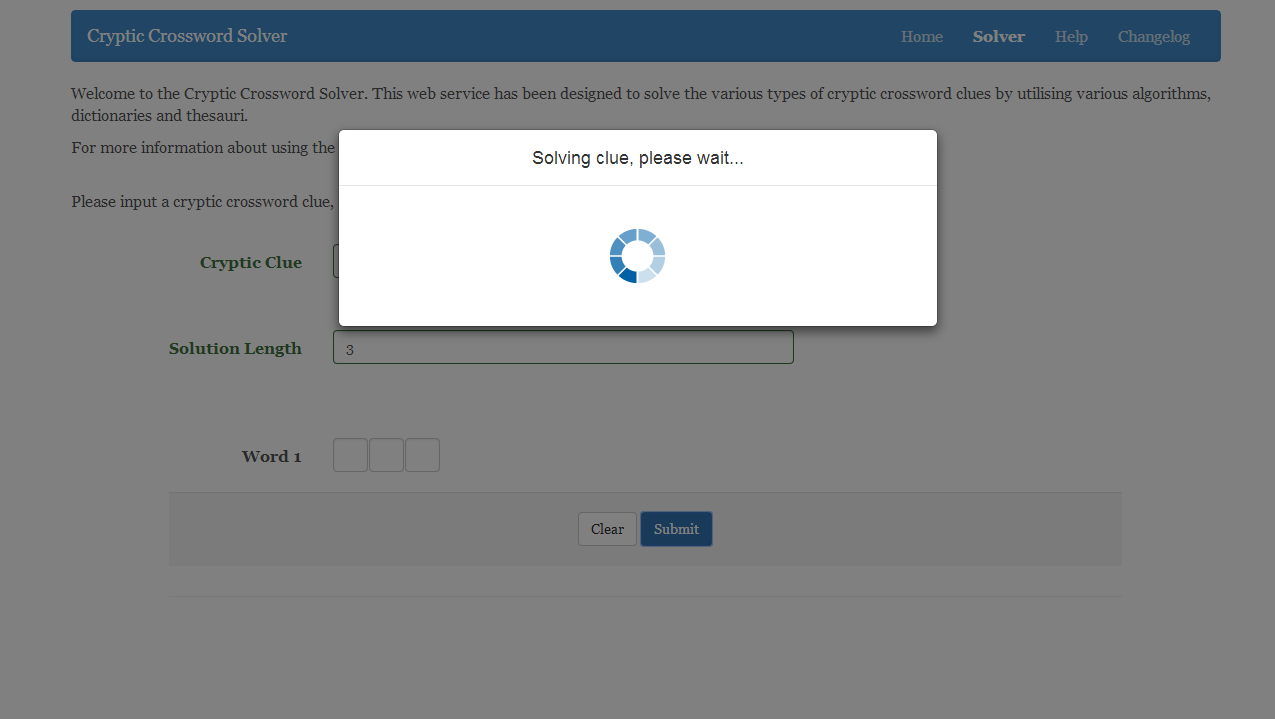
\includegraphics[width=0.9\textwidth]{images/solving_clue.png}
  \caption{Message informing the user that a clue is currently being solved}
  \label{fig:solving_clue_message}
\end{figure}

The JavaScript engine will also provide some basic forms of validation, to 
prevent the user from waiting a long time simply to find out that there was a 
validation error. The validation occurs upon a key press, and hence the feedback
is instant as shown in figure \ref{fig:validation_message}.

\begin{figure}[H]
  \centering
  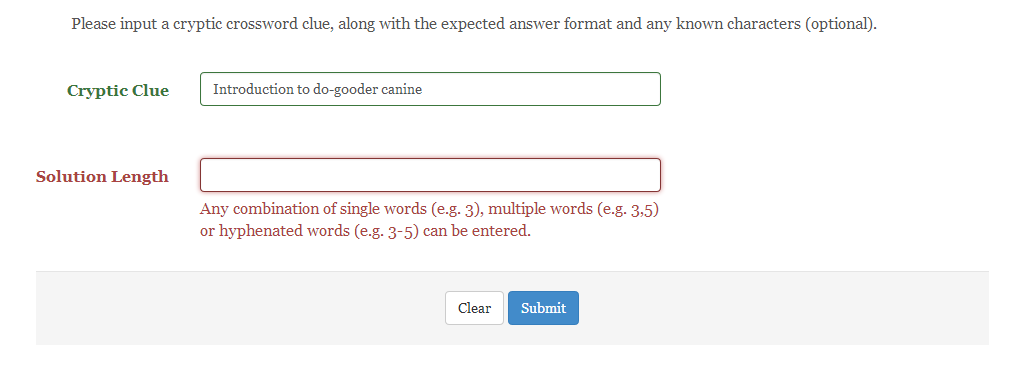
\includegraphics[width=0.9\textwidth]{images/validation.png}
  \caption{Live validation feedback ensures users are entering correct data}
  \label{fig:validation_message}
\end{figure}

The JavaScript engine will also make POST requests to the server. This reduces 
the total amount of work the server will be required to do, as it only has to 
return the requests (rather than render HTML).

The reason for the fall-back system that was previously described is that if for some reason 
the JavaScript engine fails to load, or is incompatible with the device, then 
the JavaScript will not load. However, the functionality of the site will still 
continue to work, as the browser will `fall-back' to the standard server-side 
validation and rendering.
